\chapter{Выполнение лабораторной работы №6}
\label{ch:lab6}

\section{Выбор набора данных}

Для выполнения лабораторной работы выбран набор данных \textbf{Abalone}, который содержит следующие характеристики:

\begin{itemize}
    \item Количество записей: 4177
    \item Количество признаков: 8
    \item Категориальный признак: \texttt{Sex} (M --- мужской, F --- женский, I --- детеныш)
    \item Числовые признаки: Length, Diameter, Height, Whole weight, Shucked weight, Viscera weight, Shell weight
    \item Целевая переменная: \texttt{Rings} (количество колец на раковине)
\end{itemize}

Для одномерной регрессии выбран признак \texttt{Length} (длина раковины), так как он является одним из основных измерений моллюска.

\section{Теоретическое обоснование}

Линейная регрессия — метод восстановления зависимости между двумя переменными. Пусть задана модель регрессии — параметрическое семейство функций $g(x, \alpha)$, где $\alpha \in \mathbb{R}^p$ — вектор параметров модели. Определим функционал качества аппроксимации целевой зависимости на выборке $X^\ell$ как сумму квадратов ошибок:

\[Q(\alpha, X^\ell) = \sum_{i=1}^{\ell} (g(x_i, \alpha) - y_i)^2\]

\[\alpha^* = \arg \min_{\alpha \in \mathbb{R}^p} Q(\alpha, X^\ell)\]

Стандартный способ решения этой оптимизационной задачи — воспользоваться необходимым условием минимума. Если функция $g(x, \alpha)$ достаточное число раз дифференцируема по $\alpha$, то в точке минимума выполняется система $p$ уравнений относительно $p$ неизвестных:

\[\frac{\partial Q}{\partial \alpha} (\alpha, X^\ell) = 2 \sum_{i=1}^{\ell} (g(x_i, \alpha) - y_i) \frac{\partial g}{\partial \alpha} (x_i, \alpha) = 0\]

С использованием библиотек машинного обучения эти формулы можно реализовать автоматически.

\section{Ход выполнения работы}

\subsection{Шаг 1: Загрузка и подготовка данных}

\begin{lstlisting}[language=Python, caption=Загрузка данных]
import numpy as np
import matplotlib.pyplot as plt
import pandas as pd
from sklearn.model_selection import train_test_split
from sklearn.linear_model import LinearRegression
from sklearn.metrics import mean_squared_error, r2_score

df = pd.read_csv('abalone.csv')
print(f"Размер набора данных: {df.shape}")

X = df.drop('Rings', axis=1)
y = df['Rings']

feature = 'Length'
X_simple = X[[feature]]
print(f"Признак для одномерной регрессии: {feature}")
print(f"Первые 5 значений: {X_simple[:5].values.ravel()}")
print(f"Соответствующие целевые значения: {y[:5].values}")
\end{lstlisting}

Результат выполнения:

\begin{verbatim}
Размер набора данных: (4177, 9)
Признак для одномерной регрессии: Length
Первые 5 значений: [0.455 0.35  0.53  0.44  0.33 ]
Соответствующие целевые значения: [15  7  9 10  7]
\end{verbatim}

\subsection{Шаг 2: Разделение на обучающую и тестовую выборки}

\begin{lstlisting}[language=Python, caption=Разделение данных]
X_train, X_test, y_train, y_test = train_test_split(
    X_simple, y, test_size=0.2, random_state=42
)
print(f"Размер обучающей выборки: {X_train.shape}")
print(f"Размер тестовой выборки: {X_test.shape}")
\end{lstlisting}

Результат:

\begin{verbatim}
Размер обучающей выборки: (3341, 1)
Размер тестовой выборки: (836, 1)
\end{verbatim}

Оптимальное соотношение тестовой и обучающей выборки составляет 20:80. Принцип разбиения: данные случайным образом разделяются на две непересекающиеся части; на обучающей выборке модель изучает закономерности; на тестовой выборке оценивается качество обобщения.

\subsection{Шаг 3: Обучение модели линейной регрессии}

\begin{lstlisting}[language=Python, caption=Обучение модели]
regressor = LinearRegression()
regressor.fit(X_train, y_train)
print(f"Коэффициент (наклон): {regressor.coef_[0]:.4f}")
print(f"Свободный член (интерцепт): {regressor.intercept_:.4f}")
\end{lstlisting}

Результат:

\begin{verbatim}
Коэффициент (наклон): 10.2280
Свободный член (интерцепт): 2.9950
\end{verbatim}

Метод \texttt{fit} класса \texttt{LinearRegression} вычисляет оптимальные коэффициенты модели с помощью метода наименьших квадратов, решая систему нормальных уравнений: $\beta = (X^T X)^{-1} X^T y$.

\subsection{Шаг 4: Оценка качества модели}

\begin{lstlisting}[language=Python, caption=Оценка качества]
y_pred_train = regressor.predict(X_train)
y_pred_test = regressor.predict(X_test)

train_mse = mean_squared_error(y_train, y_pred_train)
test_mse = mean_squared_error(y_test, y_pred_test)
train_r2 = r2_score(y_train, y_pred_train)
test_r2 = r2_score(y_test, y_pred_test)

print(f"\nMSE на обучающей выборке: {train_mse:.4f}")
print(f"MSE на тестовой выборке: {test_mse:.4f}")
print(f"R² на обучающей выборке: {train_r2:.4f}")
print(f"R² на тестовой выборке: {test_r2:.4f}")
\end{lstlisting}

Результат:

\begin{verbatim}
MSE на обучающей выборке: 7.0747
MSE на тестовой выборке: 7.0486
R² на обучающей выборке: 0.3312
R² на тестовой выборке: 0.3493
\end{verbatim}

\subsection{Шаг 5: Визуализация результатов}

\begin{lstlisting}[language=Python, caption=Построение графиков]
plt.figure(figsize=(12, 5))
plt.subplot(1, 2, 1)
plt.scatter(X_train, y_train, alpha=0.5, color='blue', label='Обучающие данные')
plt.plot(X_train, regressor.predict(X_train), color='red', linewidth=2, label='Линия регрессии')
plt.xlabel('Длина (Length)')
plt.ylabel('Количество колец (Rings)')
plt.title('Одномерная линейная регрессия (обучающая выборка)')
plt.legend()
plt.grid(True, alpha=0.3)

plt.subplot(1, 2, 2)
plt.scatter(X_test, y_test, alpha=0.5, color='green', label='Тестовые данные')
plt.plot(X_test, regressor.predict(X_test), color='red', linewidth=2, label='Линия регрессии')
plt.xlabel('Длина (Length)')
plt.ylabel('Количество колец (Rings)')
plt.title('Одномерная линейная регрессия (тестовая выборка)')
plt.legend()
plt.grid(True, alpha=0.3)

plt.tight_layout()
plt.savefig('lab6_univariate_regression.png', dpi=150)
print("График сохранен как 'lab6_univariate_regression.png'")
\end{lstlisting}

\begin{figure}[h]
\centering
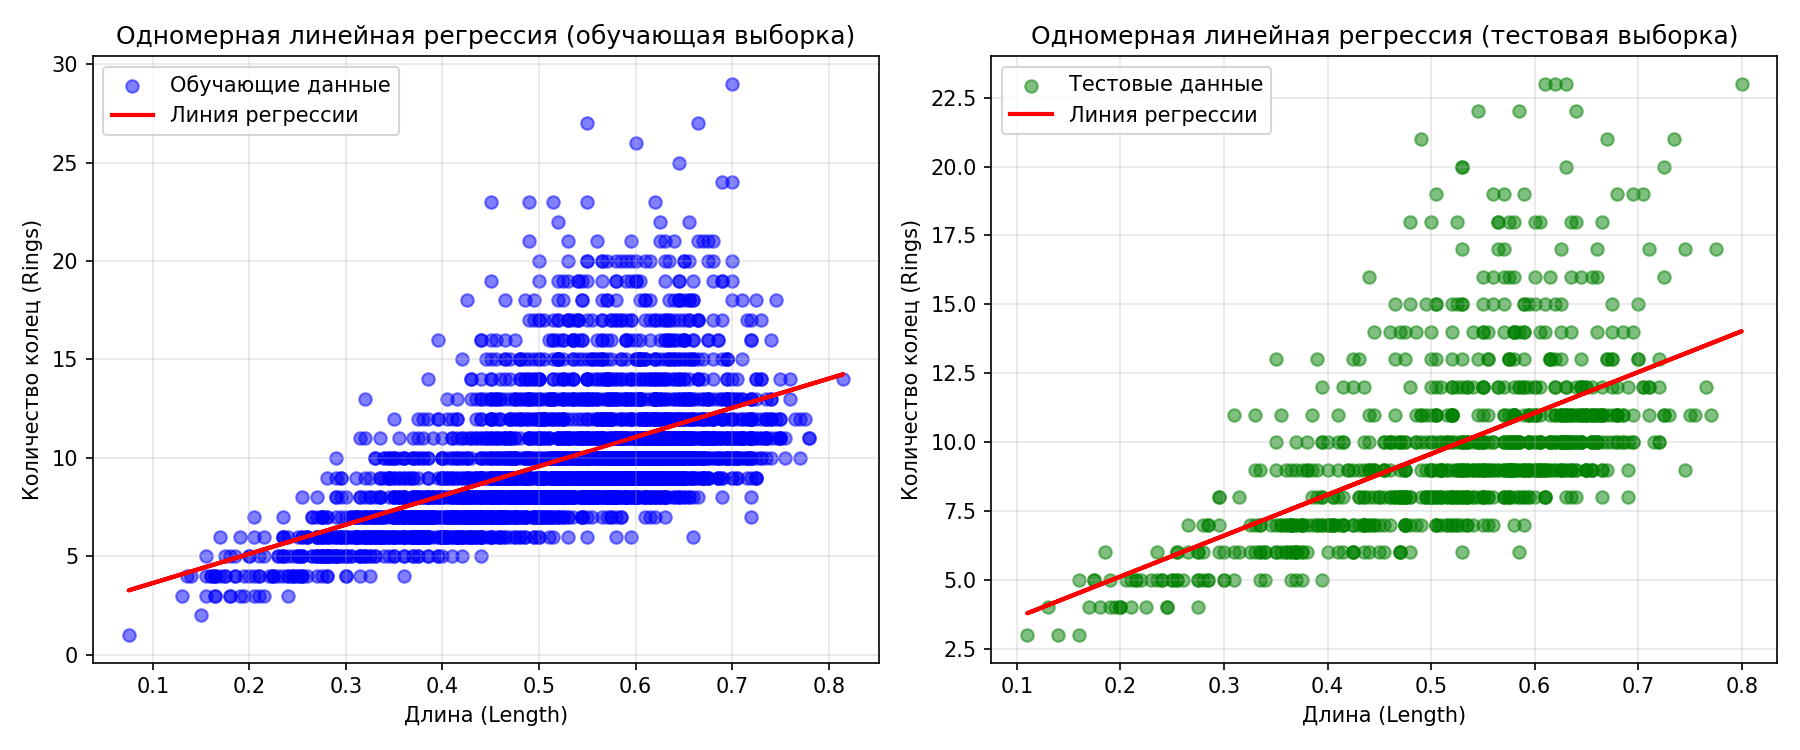
\includegraphics[width=0.9\textwidth]{lab6_univariate_regression.png}
\caption{Одномерная линейная регрессия: зависимость количества колец от длины раковины}
\label{fig:lab6_regression}
\end{figure}

\subsection{Шаг 6: Применение модели для нового объекта}

\begin{lstlisting}[language=Python, caption=Предсказание для нового объекта]
new_abalone = np.array([[0.55]])
prediction = regressor.predict(new_abalone)
print(f"\nДля моллюска с длиной 0.55 мм предсказано колец: {prediction[0]:.2f}")
print(f"Округленное значение: {int(round(prediction[0]))}")
\end{lstlisting}

Результат:

\begin{verbatim}
Для моллюска с длиной 0.55 мм предсказано колец: 8.62
Округленное значение: 9
\end{verbatim}

\section{Анализ результатов}

По результатам выполнения лабораторной работы можно сделать следующие выводы:

\begin{enumerate}
    \item Одномерная регрессия с использованием признака \texttt{Length} показала низкое качество предсказания (R² = 0.3493 на тестовой выборке).
    
    \item Коэффициент детерминации R² = 0.3493 означает, что модель объясняет только около 35\% дисперсии целевой переменной.
    
    \item Низкое качество модели объясняется слабой корреляцией между длиной раковины и количеством колец (коэффициент корреляции Пирсона составляет 0.5567).
    
    \item Среднеквадратичная ошибка (MSE) на тестовой выборке составила 7.0486, что в среднем дает ошибку предсказания около 2.65 колец (корень из MSE).
    
    \item Полученное уравнение регрессии: \texttt{Rings = 10.2280 × Length + 2.9950}.
\end{enumerate}

\section{Контрольные вопросы}

\textbf{1. Почему при реализации линейной модели регрессии нет необходимости выполнять масштабирование признаков?}

При линейной регрессии масштабирование признаков не влияет на предсказательную способность модели, так как коэффициенты модели автоматически подстраиваются под масштаб каждого признака. Если признак увеличить в $k$ раз, коэффициент уменьшится в $k$ раз, и произведение останется неизменным. Однако масштабирование может быть полезно для ускорения сходимости градиентных методов и для интерпретации коэффициентов.

\textbf{2. Почему при реализации модели линейной регрессии в качестве функции потерь используется квадратичное отклонение, а не модуль отклонения?}

Квадратичное отклонение дифференцируемо, что позволяет использовать аналитические методы оптимизации (метод наименьших квадратов) и градиентный спуск. Кроме того, оно штрафует большие ошибки сильнее, что часто желательно на практике. Функция модуля отклонения не дифференцируема в нуле, что создает проблемы при оптимизации.

\textbf{3. Что именно реализовано в методе fit(X, y) класса LinearRegression?}

Метод \texttt{fit} вычисляет оптимальные коэффициенты модели с помощью метода наименьших квадратов (MSE), решая систему нормальных уравнений: $\beta = (X^T X)^{-1} X^T y$. Для этого используется численно устойчивая реализация на основе сингулярного разложения (SVD).

\textbf{4. Что такое p-значение? Как p-значение используется при оптимизации моделей регрессии?}

P-значение — это вероятность получить наблюдаемый результат при условии, что нулевая гипотеза верна. В регрессии p-значение для коэффициента показывает, значимо ли отличается коэффициент от нуля. Обычно признаки с $p > 0.05$ считаются незначимыми и могут быть удалены из модели.

\textbf{5. Поясните назначение метода predict класса LinearRegression.}

Метод \texttt{predict} вычисляет предсказанные значения целевой переменной для новых данных на основе обученной модели: $\hat{y} = X\beta$. Для каждого объекта из входной матрицы $X$ вычисляется линейная комбинация признаков с весами-коэффициентами.

\textbf{6. Поясните назначение метода plot и scatter класса pyplot.}

Метод \texttt{scatter} строит диаграмму рассеяния — отображает точки с координатами (x, y). Метод \texttt{plot} строит линейный график, соединяя точки отрезками. В данной работе \texttt{scatter} использовался для отображения реальных данных, а \texttt{plot} — для отображения линии регрессии.

\textbf{7. По какой подвыборке необходимо оценивать точность модели машинного обучения: тестовой или тренировочной?}

Точность модели необходимо оценивать по тестовой выборке, так как она не участвовала в обучении и позволяет оценить способность модели к обобщению на новых, ранее не виденных данных. Оценка по обучающей выборке может быть завышена из-за переобучения.

\section{Листинг программы}

\lstinputlisting[language=Python, caption=Полный код лабораторной работы №6]{lab6.py}

\section*{Вывод}

В ходе выполнения лабораторной работы №6 был разработан пайплайн для решения задачи одномерной регрессии. На основе набора данных Abalone была построена модель линейной регрессии для предсказания количества колец по длине раковины.

Полученные результаты:
\begin{itemize}
    \item Уравнение регрессии: \texttt{Rings = 10.2280 × Length + 2.9950}
    \item Коэффициент детерминации R² = 0.3493
    \item Среднеквадратичная ошибка MSE = 7.0486
\end{itemize}

Модель показала низкое качество предсказания, что объясняется слабой корреляцией между выбранным признаком и целевой переменной. Для улучшения качества необходимо использовать многомерную регрессию с несколькими признаками. Все поставленные задачи выполнены.

\endinput